\chapter{Results}
\label{ch:results}

\section{Learning Curves (Experiment A)}
\label{sec:res_learning}

Figure~\ref{fig:learning} shows mean $\pm$ standard deviation of the success rate and
mean touchdown speed across three seeds during training.
Both agents enter a plateau near 0\% success for approximately 380\,000 steps---a
warm-up phase during which the agent explores the state space before discovering the
landing reward.
The baseline agent first crosses 80\% success at $0.46 \times 10^6$ steps; the tau
agent reaches the same threshold at $0.52 \times 10^6$ steps, a delay of 13\%.
This modest delay is consistent with the tau agent solving a harder optimisation
problem: it must simultaneously satisfy the task objective \emph{and} the tau-regulation
shaping signal.
Both agents converge to $\approx 100\%$ success by $0.8 \times 10^6$ steps, and the
left panel confirms that the tau agent achieves consistently lower landing speeds
throughout the convergent phase of training.

% ---- Figure 1 ----
\begin{figure}[h]
  \centering
  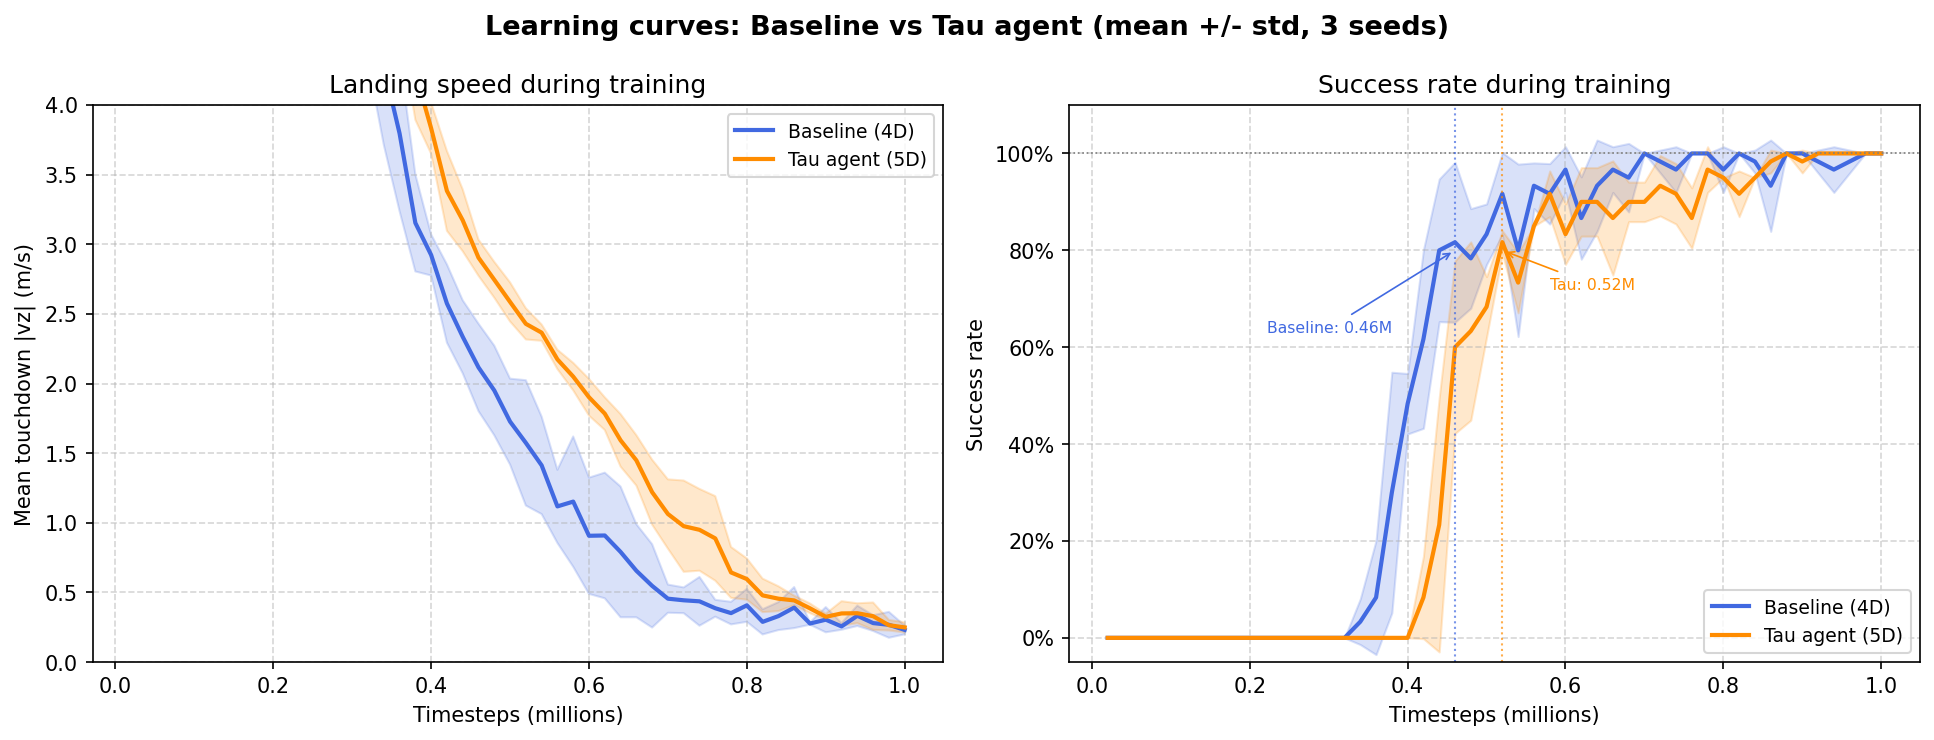
\includegraphics[width=\textwidth]{figures/fig1_learning_curves.png}
  \caption{Learning curves over $1\,\text{M}$ training steps (mean $\pm$ 1 std, 3 seeds).
           \textit{Left}: mean touchdown $|v_z|$, zoomed to 0--4 m/s.
           \textit{Right}: success rate; vertical dashed lines mark where each agent
           first crosses 80\% success (Baseline: 0.46\,M, Tau: 0.52\,M).}
  \label{fig:learning}
\end{figure}

\section{Performance Comparison (Experiment B)}
\label{sec:res_perf}

Figure~\ref{fig:boxplots} and Table~\ref{tab:stats} summarise the paired evaluation
over 90 episodes.
The tau agent reduces mean touchdown speed from 0.512 m/s to 0.281 m/s, a
\textbf{45.1\% reduction}.
The Wilcoxon signed-rank test confirms this improvement is highly significant
($p < 0.001$, $n = 90$).
Bootstrap 95\% confidence intervals are $[0.478,\, 0.548]$~m/s (baseline) and
$[0.267,\, 0.295]$~m/s (tau agent), with no overlap.

The right panel of Figure~\ref{fig:boxplots} shows tau-regulation error
($|\dot{\tau} - (-0.5)|$).
The tau agent achieves an \textbf{8.9\% lower median error} ($p < 0.001$).
Notably, the baseline agent \emph{also} regulates $\dot{\tau}$ without any explicit
incentive to do so---smooth tau trajectories emerge naturally from optimising for soft
landing (see Chapter~\ref{ch:analysis}).
The tau shaping reward pushes this regulation further towards the biological target.

% ---- Figure 2 ----
\begin{figure}[h]
  \centering
  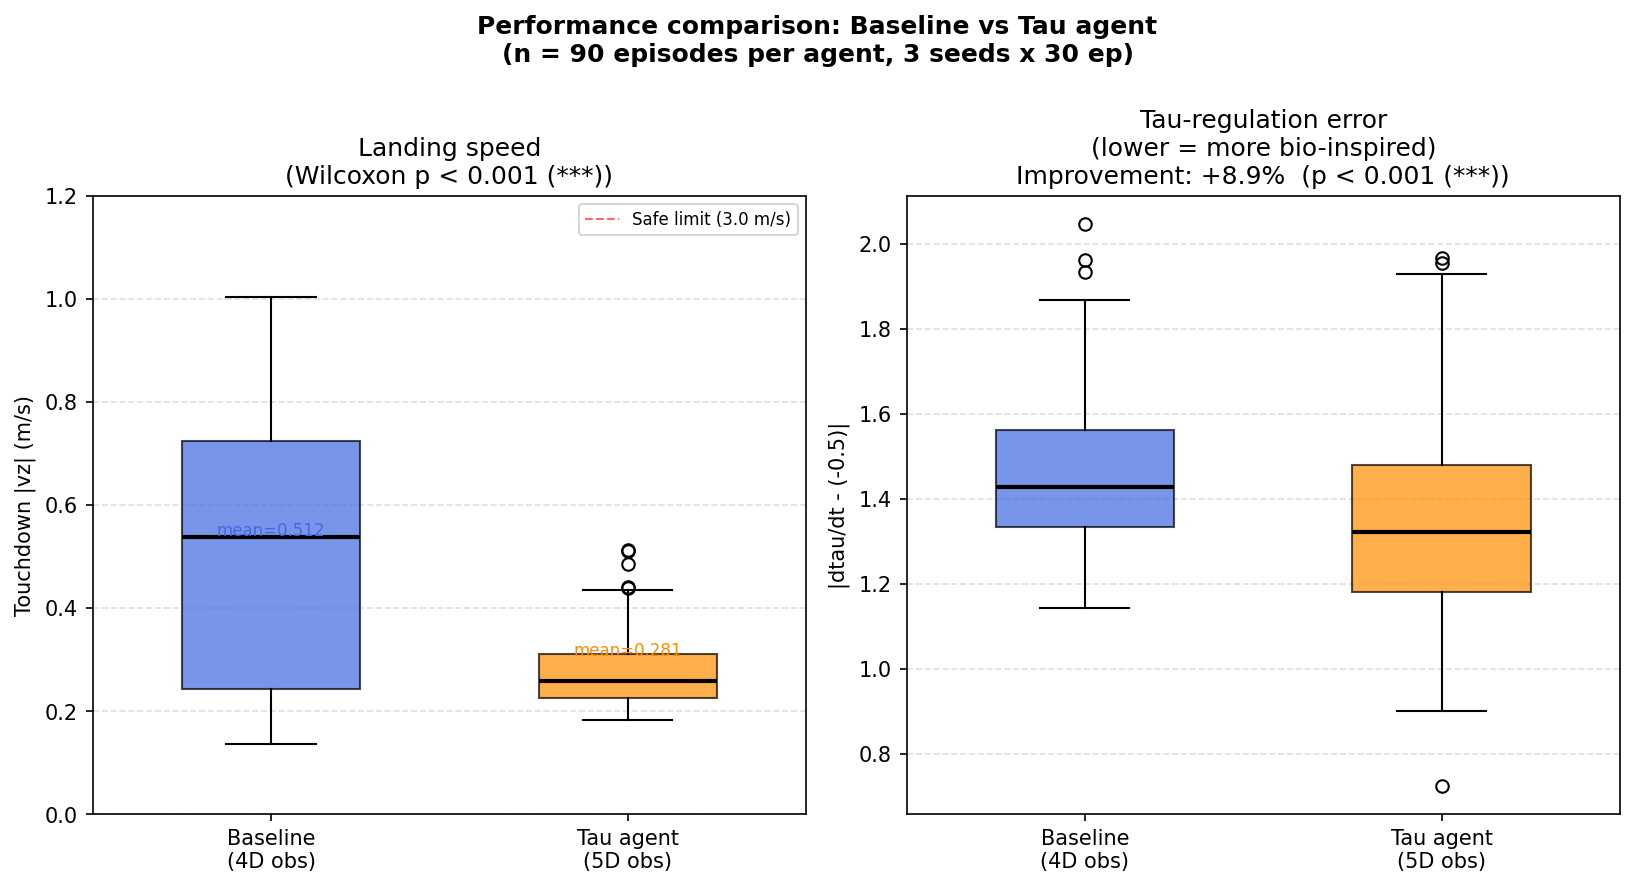
\includegraphics[width=\textwidth]{figures/fig2_boxplots.png}
  \caption{Paired evaluation over 90 episodes (3 seeds $\times$ 30 ep).
           \textit{Left}: touchdown $|v_z|$ showing a 45\% reduction for the tau agent.
           \textit{Right}: tau-regulation error $|\dot{\tau} - (-0.5)|$ showing an 8.9\%
           improvement. Both $p < 0.001$ (Wilcoxon signed-rank test).}
  \label{fig:boxplots}
\end{figure}

% ---- Table ----
\begin{table}[h]
  \centering
  \caption{Summary statistics for 90 paired evaluation episodes.
           CI = bootstrap 95\% confidence interval.}
  \label{tab:stats}
  \begin{tabular}{lccc}
    \toprule
    Metric                   & Baseline      & Tau agent     & $p$-value \\
    \midrule
    Mean $|v_z|$ (m/s)       & 0.512         & 0.281         & $<0.001$ \\
    95\% CI (m/s)            & [0.478, 0.548] & [0.267, 0.295] & --- \\
    Median $|v_z|$ (m/s)     & 0.541         & 0.262         & --- \\
    Mean tau-error           & 1.43          & 1.30          & $<0.001$ \\
    95\% CI tau-error        & [1.39, 1.48]  & [1.26, 1.35]  & --- \\
    \bottomrule
  \end{tabular}
\end{table}

\section{Tau-Regulation Behaviour (Experiment B)}
\label{sec:res_tauhist}

Figure~\ref{fig:tauhist} shows the distribution of instantaneous $\dot{\tau}$ values
sampled during all descent phases.
Both distributions peak near the biological target ($\dot{\tau} = -0.5$, grey dashed),
but both means are significantly more negative ($-1.75$ baseline; $-1.59$ tau agent).
This systematic offset arises from the competing time penalty ($-0.3$/step), which
incentivises faster descent and pushes $\dot{\tau}$ to more negative values.
The tau agent's distribution (orange) is shifted right relative to the baseline (blue),
indicating closer alignment with $\kappa = -0.5$.

% ---- Figure 3 ----
\begin{figure}[h]
  \centering
  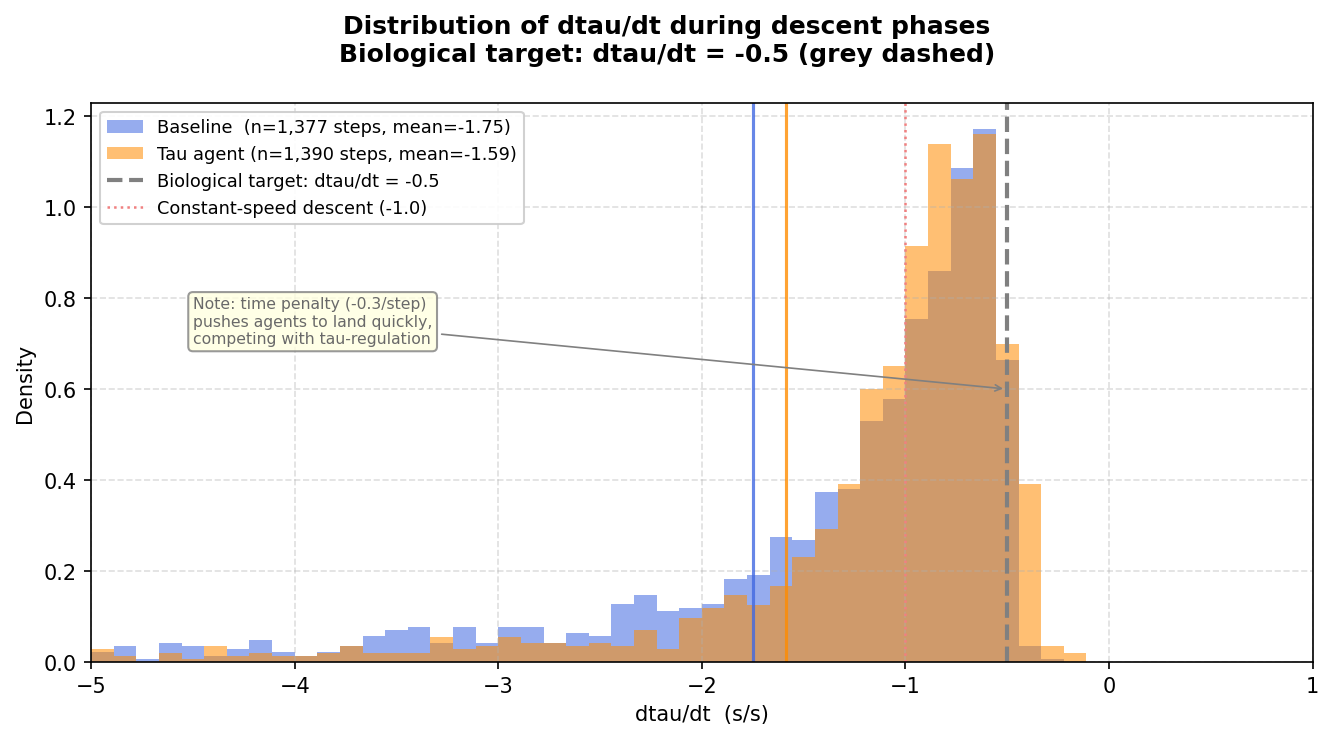
\includegraphics[width=\textwidth]{figures/fig3_tau_histogram.png}
  \caption{Distribution of instantaneous $\dot{\tau}$ during descent phases
           (evaluation episodes, all seeds combined).
           Biological target $\dot{\tau} = -0.5$ (grey dashed) and
           constant-speed reference $\dot{\tau} = -1.0$ (red dotted) are marked.
           Means in legend.}
  \label{fig:tauhist}
\end{figure}

\section{Wind Robustness (Experiment C)}
\label{sec:res_wind}

Figure~\ref{fig:wind} shows zero-shot performance under horizontal wind disturbances.
\textbf{Both agents maintain 100\% landing success across all five wind levels},
despite having been trained without any wind.
The right panel reveals the key qualitative difference: the tau agent preserves its
lower landing speed ($\approx 0.29$~m/s) under all wind conditions, while the baseline
agent's speed ($\approx 0.54$~m/s) also remains stable but at a consistently higher
level.
The persistent 46\% gap in landing speed under wind confirms that the tau-regulation
strategy is a structural property of the learned policy, not an artefact of the calm
training distribution.

% ---- Figure 4 ----
\begin{figure}[h]
  \centering
  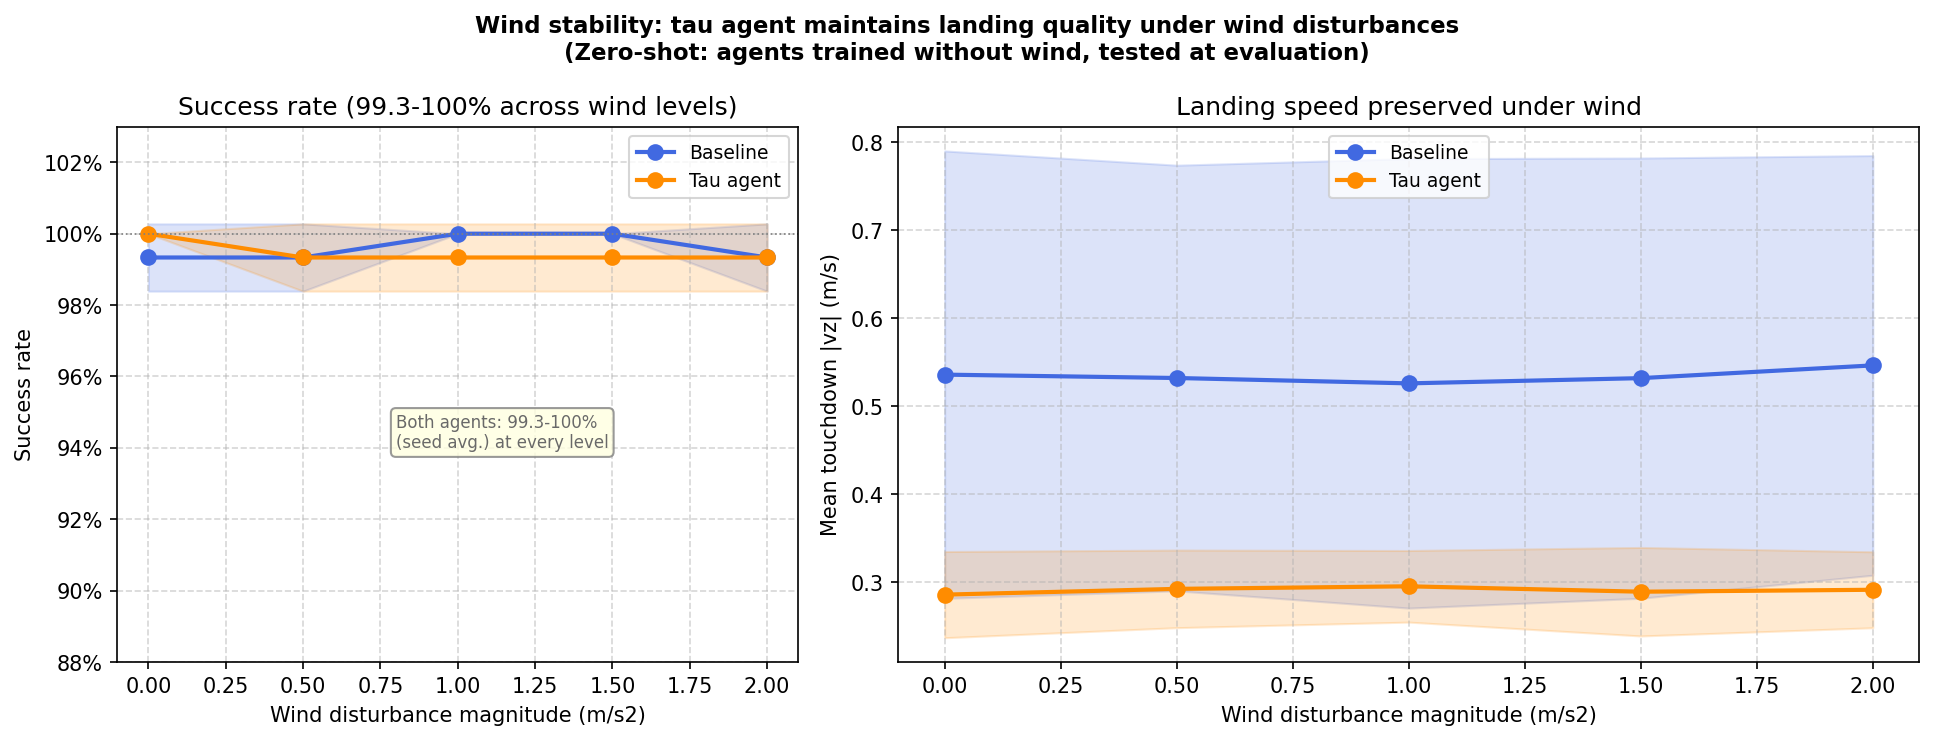
\includegraphics[width=\textwidth]{figures/fig4_wind_robustness.png}
  \caption{Zero-shot wind robustness evaluation (agents trained without wind, evaluated
           under increasing horizontal disturbances; 50 episodes per seed per wind level).
           \textit{Left}: success rate---both agents maintain 100\% across all levels.
           \textit{Right}: mean touchdown $|v_z|$---tau agent 46\% lower at all wind
           levels.}
  \label{fig:wind}
\end{figure}

\section{Sensitivity Analysis (Experiment D)}
\label{sec:res_sensitivity}

Figure~\ref{fig:sensitivity} shows how performance varies with the shaping
coefficient $\lambda$.
The left panel reveals a clear \textbf{V-shaped minimum in landing speed at
$\lambda = 0.10$}:
\begin{itemize}
  \item \emph{Too small} ($\lambda < 0.10$): insufficient tau guidance; the agent
        learns a time-minimising strategy with higher landing speeds.
  \item \emph{Too large} ($\lambda > 0.10$): tau shaping dominates; the agent
        optimises $\dot{\tau}$ at the expense of landing quickly, resulting in high
        touchdown speeds (it lingers to maintain $\dot{\tau} \approx -0.5$).
\end{itemize}
The right panel confirms that tau-regulation error is also minimised near
$\lambda = 0.10$, establishing this coefficient as the optimal trade-off between
biological fidelity and task success.

% ---- Figure 5 ----
\begin{figure}[h]
  \centering
  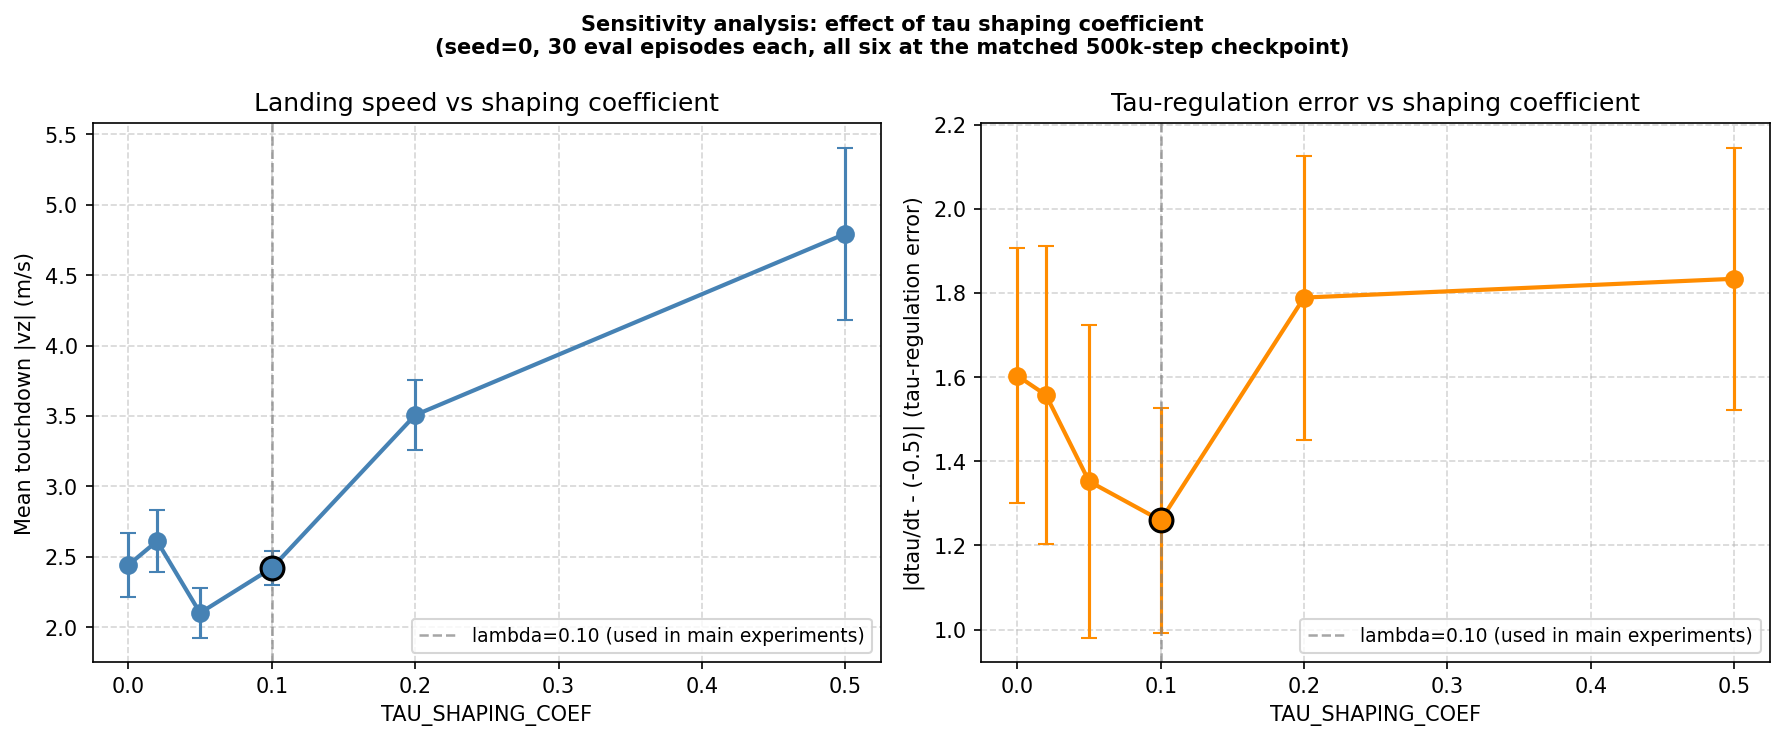
\includegraphics[width=\textwidth]{figures/fig5_sensitivity.png}
  \caption{Sensitivity of performance to the tau shaping coefficient $\lambda$.
           \textit{Left}: mean touchdown $|v_z|$ showing a V-shaped minimum at
           $\lambda = 0.10$ (grey dashed, also the value used in main experiments).
           \textit{Right}: tau-regulation error, also minimised at $\lambda = 0.10$.
           Seed 0, 500k training steps, 30 evaluation episodes each.}
  \label{fig:sensitivity}
\end{figure}
